\subsection{QuizziPedia::Front-End}
\subsubsection{Informazioni generali}
\label{QuizziPedia::Front-End}
\begin{figure}[ht]
	\centering
	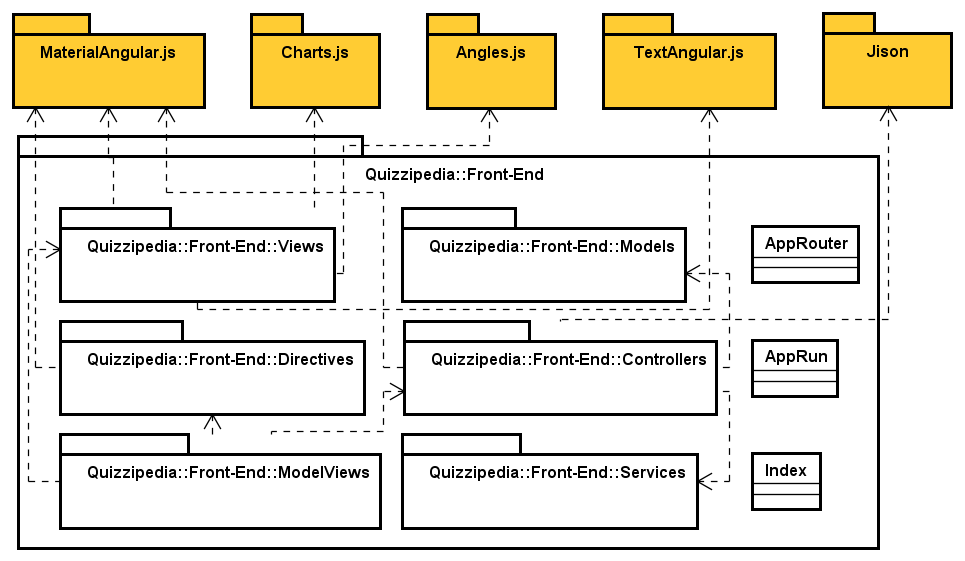
\includegraphics[scale=0.45]{UML/Package/QuizziPedia_Front-end.png}
	\caption{QuizziPedia::Front-End}
\end{figure}
\FloatBarrier
	\begin{itemize}
		\item \textbf{Descrizione}: package contenente le componenti front-end dell'applicazione.
		\item \textbf{Package contenuti}:
		\begin{itemize}
			\item \texttt{Controllers}: package contenente i controllers front-end dell'applicazione.
			\item \texttt{Directives}: package contenente le directives front-end dell'applicazione.
			\item \texttt{Models}: package contenente le classi che definiscono la business logic dell'applicazione.
			\item \texttt{Services}: package contenente i services front-end dell'applicazione.
			\item \texttt{Views}: package contenente le views front-end dell'applicazione.
			\item \texttt{Templates}: package contenente i templates front-end dell'applicazione.
		\end{itemize}
	\end{itemize}

\subsubsection{Classi}
	\paragraph{QuizziPedia::Front-End::AppRouter}
	
	\label{QuizziPedia::Front-End::AppRouter}
	
	\begin{figure}[ht]
		\centering
		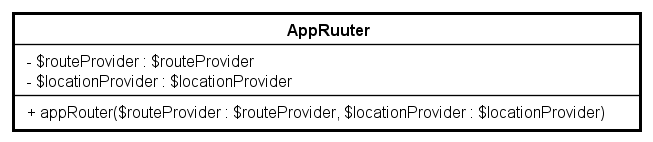
\includegraphics[scale=0.5,keepaspectratio]{UML/Classi/Front-End/QuizziPedia_Front-end_AppRouter.png}
		\caption{QuizziPedia::Front-End::AppRouter}
	\end{figure} \FloatBarrier
	
	\begin{itemize}
		\item \textbf{Descrizione}: classe che gestisce i routes dell’applicazione, utilizza il servizio \$routeProvider per associare ad ogni route un controller e una view;
		\item \textbf{Utilizzo}: viene utilizzata per associare un URL alle varie view dell’applicazione;
		\item \textbf{Metodi}: 
		\begin{itemize}
			\item \texttt{-} \texttt{appRouter(\$routeProvider: \$routeProvider, \$locationProvider: \$locationProvider)}: metodo che gestisce i routes dell’applicazione. Utilizza il servizio \$routeProvider per associare ad ogni route un controller e una view; e \$locationProvider per configurare come i paths dell'applicazione vengono salvati. Questa funzione viene utilizzata come parametro nel metodo texttt{config} di \textit{Angular.js}. Il metoto \texttt{config} permette di impostare l'esecuzione di una funzione al caricamento del \textit{modulo\ped{G}} principale di \textit{Angular.js\ped{G}};
			\textbf{Metodi}:
			\begin{itemize}
				\item \texttt{\$routeProvider}: campo dati contenente un riferimento al servizio di \textit{Angular.js\ped{G}} che si occupa di definire le route dell’applicazione;
				\item \texttt{\$locationProvider}: campo dati contenente un riferimento al servizio di \textit{Angular.js\ped{G}} che si occupa di configuare come i paths vengono memorizzati;
			\end{itemize}
		\end{itemize}
	\end{itemize}
	
	\paragraph{QuizziPedia::Front-End::AppRun}
	
	\label{QuizziPedia::Front-End::AppRun}
	
	\begin{figure}[ht]
		\centering
		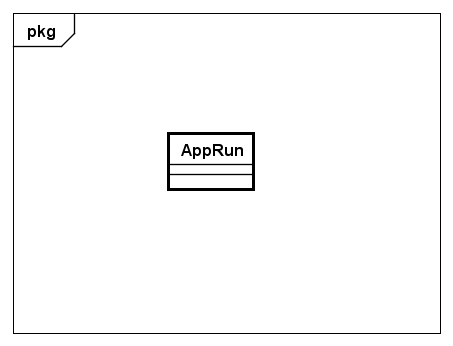
\includegraphics[scale=0.5,keepaspectratio]{UML/Classi/Front-End/QuizziPedia_Front-end_AppRun.png}
		\caption{QuizziPedia::Front-End::AppRun}
	\end{figure} \FloatBarrier
	
	\begin{itemize}
		\item \textbf{Descrizione}: classe che verifica se l'utente sia autenticato e che abbia le giuste autorizzazioni per la pagina in cui si trova;
		\item \textbf{Utilizzo}: viene utilizzata per verificare che l’utente sia autenticato e che abbia la giusta autorizzazione per la pagina in cui si trova;
		\item \textbf{Relazioni con altre classi}: 
		\begin{itemize}
			\item \textit{IN} \texttt{}: ; 
		\end{itemize}
		\item \textbf{Attributi}: 
		\begin{itemize}
			\item ;
		\end{itemize}
		\item \textbf{Metodi}: 
		\begin{itemize}
			\item ;
		\end{itemize}
	\end{itemize}
	
	\paragraph{QuizziPedia::Front-End::Index}
	\begin{itemize}
		\item \textbf{Descrizione}: view generale dell'applicazione;
		\item \textbf{Utilizzo}: contiene gli elementi che saranno presenti in ogni pagina dell'applicazione;
		\item \textbf{Relazioni con altre classi}:
		\begin{itemize}
			\item \textit{IN} \texttt{MenuBarDirective}: rappresenta il menù, presente in ogni pagina dell'applicazione, generato in base agli oggetti passati nello \$scope isolato. Fornisce un pulsante per ogni oggetto ricevuto come parametro, ogni pulsante viene rappresentato con un’icona e con un testo. Al click di un pulsante viene invocata la funzione ad esso associata;
			\item \textit{IN} \texttt{ErrorsDirective}: directive che mostra l'eventuale errore dopo un'azione;
			\item \textit{IN} \texttt{FooterDirective}: directive che mostra il footer dell'applicazione che sarà presente in ogni pagina;
		\end{itemize}
		\item \textbf{Attributi}
	\end{itemize}